\rs{This section deals with the single \Xi\ spectra check I did to make sure the normalisation (and all things contributing to it) were correct. I think this can be split into 2 parts: the different efficiency correction related to the ``event factor'', and the actual results. This section is still a pretty rough draft.}

[this is a small introduction]

We performed a short analysis on the single \Xi\ spectra. This was motivated by the discrepancy between the results presented in this thesis and the analysis performed on data gathered in the previous data-taking period (Run 2). \cite{Adolfson2024} 

\rs{Not sure how to motivate this in a ``politically correct'' way, but a large part of the motivation for this check is that the discrepancy between run 2 and 3 is flat in dphi - which indicates a normalisation issue. By analyzing the single particle spectrum, we can more or less verify the normalisation.}

Studying the single particle spectra of cascades is interesting in it's own right, as can be seen from publications such as (but not limited to) the Nature article on strangeness enhancement \cite{StrangenessEnhancement} discussed in Section \ref{sec:theory:strangeness_enhancement}. In this analysis we will present the yield of \Xi\ baryons as a function of \pt\, which serves as both a stepping stone to producing correlations between \Xi\ baryons as well as an important cross-check to validate the correlation results. After all, when one wants to analyse observables involving multiple \Xi\ baryons, one better make sure that the single \Xi\ spectra are correct. 

\section{Efficiency corrections for \texorpdfstring{\Xi}{Xi} baryon yields}

  The \Xi\ baryon yields are calculated according to the following equation:
  \begin{align}
    \frac{1}{N^\text{true}_\text{events}} \frac{\d^2 N_\Xi}{\d\pt \d\y} = \frac{\epsilon_\text{event}}{N^\text{rec.}_\text{events}} \frac{N^\text{rec.}_\text{casc.}(\pt, \y)}{\epsilon_\text{\Xi}(\pt, \eta) \Delta \pt \Delta \y}, \label{eq:single_spectra}
  \end{align}

  where $\epsilon_\text{event}$ is the event reconstruction efficiency and $\epsilon_\text{\Xi}(\pt, \eta)$ is the cascade reconstruction efficiency. As we report the yield in the central rapidity window $|\y| < 0.5$, $\Delta \y = 0.5 - (-0.5) = 1$ and drops out of the equation. Note that to be consistent with the correlation analysis we apply the efficiency correction as a function of \eta\ rather than \y\, as we require both the generated and reconstructed cascade to be within $|\eta| < 0.8$. Combining such an \eta\ selection with an efficiency correction as a function of \y\ would lead to unwanted edge effects in the efficiency correction. 

  The \Xi\ efficiency correction is different for single particle yields compared to correlation studies. This is due to the fact that in correlation studies we are interested in quantities \textit{per trigger}, whereas in single particle spectra we are interested in quantities \textit{per event}. This results in a slightly different definition of the cascade reconstruction efficiency that can be written as:
  \begin{align}
    \epsilon(\pt, \eta) = \frac{N^\text{rec.}_\Xi(\pt, \eta)}{N^\text{gen.}_\Xi(\pt, \eta)}. \label{eq:efficiency_spectra}
  \end{align}

  Compared to the efficiency correction for correlation studies given by Equation \ref{eq:efficiency}, we no longer require that a generated cascade has a matched reconstructed event, as efficiency loss due to event loss is something we want to account for. Note that we do require that the generated event is reconstructible, i.e. that the generated event passes our event selections. However, some of our event selections such as the \texttt{sel8} selection criterium are based on reconstructed level information, and we by definition do not have access to this information at the generated level. So we only apply the event selections that can be defined at the generated level, albeit slightly different from the reconstructed level due to fundamental differences between generated and reconstructed information. This consists of two different event selections:
  \begin{itemize}
    \item $V_z < 10$ cm: as the position of the primary vertex is available at the generated level, this is a rather straightforward analogy to the reconstructed level selection.
    \item INEL$>$0: at the reconstructed level this selection is applied at track level by requiring at least one central charged track that contributes to the PV. The generated level equivalent is to require at least one charged primary particle within $|\eta| < 0.8$. 
  \end{itemize}

  The event reconstruction efficiency is needed to account for any event loss that affects the per-event normalisation. It is given by 
  \begin{align}
    \epsilon_\text{event} = \frac{N^\text{gen.}_\text{events}}{N^\text{rec.}_\text{events}}. \label{eq:event_efficiency}
  \end{align}

  Also here we require that the generated event is reconstructible, so we only consider generated events that pass the generated level event selections described above. Note that the event efficiency is not dependent on any properties of the \Xi\ baryons, and should therefor only impact the overal normalisation of the spectra, not the shape. The efficiency corrections as a function of \pt\ and \eta\ are shown in Figure \ref{fig:SpectraEff2D}, with projections on the \pt\ axis shown in Figure \ref{fig:SpectraEffPt}. 

  \begin{figure}[ht]
    \centering
    \begin{subfigure}[t]{.49\textwidth}
      \centering
      \includegraphics[width=\textwidth]{figures/Intermezzo/Efficiency/2D/hXiMinEff.pdf}
      \caption{$\Xi^-$ efficiency}
      \label{fig:SpectraXiMinEff}
    \end{subfigure}
    \hfill
    \begin{subfigure}[t]{.49\textwidth}
      \centering
      \includegraphics[width=\textwidth]{figures/Intermezzo/Efficiency/2D/hXiPlusEff.pdf}
      \caption{$\Xi^+$ efficiency}
      \label{fig:SpectraXiPlusEff}
    \end{subfigure}
    \caption{Efficiency corrections for the single \Xi\ spectra.}
    \label{fig:SpectraEff2D}
  \end{figure}

  \begin{figure}[ht]
    \centering
    \begin{subfigure}[t]{.49\textwidth}
      \centering
      \includegraphics[width=\textwidth]{figures/Intermezzo/Efficiency/1D/hPtXiMinEff.pdf}
      \caption{$\Xi^-$ efficiency}
      \label{fig:SpectraXiMinEffPt}
    \end{subfigure}
    \hfill
    \begin{subfigure}[t]{.49\textwidth}
      \centering
      \includegraphics[width=\textwidth]{figures/Intermezzo/Efficiency/1D/hPtXiPlusEff.pdf}
      \caption{$\Xi^+$ efficiency}
      \label{fig:SpectraXiPlusEffPt}
    \end{subfigure}
    \caption{Efficiency corrections for the single \Xi\ spectra as a function of \pt.}
    \label{fig:SpectraEffPt}
  \end{figure}

\section{Systematic uncertainties for \texorpdfstring{\Xi}{Xi} baryon yields}
  To investigate any potential sources of discrepancies or systematic uncertainties, we started by looking into the distributions of the topological variables used in the cascade selection. Any non-trivial selection on these variables will lead to a different reconstruction efficiency. In order to accurately model this, the distributions of the topological variables should be well described by the Monte Carlo simulations used to determine the efficiency corrections, even before applying the selection on these variables. It is computationally not feasible to consider all possible cascade candidates before applying any selection, as this is equivalent to considering all possible track triplet combinations in an event. Therefore, we apply a set of `minimal' selection criteria before looking at the distributions of the topological variables. In principle these selection criteria aim to be as inclusive as possible while reducing the combinatorial background by requiring a minimum distance of all daughter tracks to the primary vertex. These minimal selection criteria are shown in Table \ref{tab:minsel}.

  \begin{table}[ht]
    \centering
    \begin{tabular}{|c|c|}
      \hline
      \multicolumn{2}{|c|}{Minimal selection criteria} \\
      \hline
      $|\eta_\text{tracks}|$ & $< 0.8$ \\
      \hline
      Number of TPC crossed rows & $> 50$ \\
      \hline
      DCA V0 daughters & $< 1.0$ \\
      \hline
      DCA cascade daughters & $< 1.0$ \\
      \hline
      DCA pos V0 daughter to PV & $> 0.01$ \\
      \hline
      DCA neg V0 daughter to PV & $> 0.01$ \\
      \hline
      DCA bach to PV & $> 0.02$ \\
      \hline
      V0 $\cos(\text{PA})$ & $> 0.97$ \\
      \hline
      Cascade $\cos(\text{PA})$ & $> 0.97$ \\
      \hline
      V0 radius & $> 0.5$ \\
      \hline
      Cascade radius & $> 0.5$ \\
      \hline
      V0 mass window & $< 14$ MeV/$c^2$\\
      \hline
    \end{tabular}
    \caption{Minimal selection criteria for cascade candidates}
    \label{tab:minsel}
  \end{table}

  We compare the distributions of some topological variables after applying the minimal selection criteria on both data and Monte Carlo simulations. In the case of the MC simulations we require that the reconstructed cascade is matched to a generated cascade, while in the data sample we apply a rough invariant mass selection of 1.31 \gev $< m_\text{inv} <$ 1.33 \gev to limit the contribution of combinatorial background. We also self-normalise the distributions to account for the difference in statistics between the two samples. Three topological variables seemed to exhibit particular discrepancies between data and MC simulations: DCA of the V0 (\Lambda) to the PV, DCA of the V0 daughters to the PV, and the cascade radius. In all three cases the selection criterium is a minimum value. The distributions of these variables are shown in Figure \ref{fig:TopologicalDistributions}, where the DCA of the V0 daughters are split by charge. 

  \begin{figure}
    \centering
    \begin{subfigure}[t]{.49\textwidth}
      \centering
      \includegraphics[width=\textwidth]{figures/Intermezzo/systematics/Before_hDCAV0ToPV.pdf}
      \caption{DCA of the V0 to the PV}
      \label{fig:DCAV0ToPV}
    \end{subfigure}
    \hfill
    \begin{subfigure}[t]{.49\textwidth}
      \centering
      \includegraphics[width=\textwidth]{figures/Intermezzo/systematics/Before_hDCAPosToPV.pdf}
      \caption{DCA of the positive V0 daughter to the PV}
      \label{fig:DCAPosToPV}
    \end{subfigure}
    \hfill
    \begin{subfigure}[t]{.49\textwidth}
      \centering
      \includegraphics[width=\textwidth]{figures/Intermezzo/systematics/Before_hDCANegToPV.pdf}
      \caption{DCA of the negative V0 daughter to the PV}
      \label{fig:DCANegToPV}
    \end{subfigure}
    \hfill
    \begin{subfigure}[t]{.49\textwidth}
      \centering
      \includegraphics[width=\textwidth]{figures/Intermezzo/systematics/Before_hCascRadius.pdf}
      \caption{Cascade radius}
      \label{fig:CascRad}
    \end{subfigure}

    \caption{Distributions of topological variables for data and MC simulations after applying the minimal selection criteria. The distributions are self-normalised to account for differences in statistics between the two samples. The DCA of the V0 daughters to the PV are split by charge. }
    \label{fig:TopologicalDistributions}
  \end{figure}

  The DCA of the V0 to the PV (\texttt{DCAV0ToPV}) differs between data and MC across a rather large range of values - any reasonable minimum value should lie between 0 and 0.1 cm, which covers the range where the discrepancy is observed. Instead of assessing the impact of this discrepancy we decide to do away with this selection criterium altogether. This is motivated in part by the fact that a reasonable cut on this variable would not discard a large fraction of the sample. 
  
  The DCA of the V0 daughters to the PV (\texttt{DCAPosToPV}, \texttt{DCANegToPV}) also shows a discrepancy between data and MC across a large range of values, including the region where any reasonable selection criterium would lie. To investigate the effect of this discrepancy on the \pt\ distribution of the \Xi\ baryons we vary the minimum value of this selection criterium significantly with three values: 0.01 cm, 0.20 cm, and 0.30 cm. These values are chosen to cover as much of the range of the discrepancy as possible without discarding too much of the available statistics. As this criterium works on the track level (not the \Xi\ candidate level), large minimum values will lead to a significant drop of reconstruction efficiency. To compare the different variations we copmute the \Xi\ \pt\ spectrum for each of the three variations, and look at the ratio of the lowest and highest variations to the middle variation. The results are shown in Figure \ref{fig:SpectraRatioDCAPosNegToPV}, where the uncertainties are calculated assuming they are fully correlated between the variations. The weighted averages show that the effect is rather small, with the smallest effect observed when comparing the 0.20 and 0.30 cm variations. Combining this with the fact that large minimum values for this variable lead to a significant drop in reconstruction efficiency, we decide to use 0.05 as the default value, with variations of 0.01 and 0.10 to estimate the systematic uncertainty as part of the ensemble variation. 

  \begin{figure}
    \centering
    \includegraphics[width=.8\textwidth]{figures/Intermezzo/systematics/spectra_ratio_DCAPosNegToPV.pdf}
    \caption{Ratio of the \Xi\ \pt\ spectra for different variations of the minimum DCA of the V0 daughters to the PV. The vertical bars represent the statistical uncertainties subtracted in quadrature, assuming they are fully correlated between the variations. The weighted average of the ratios are also drawn as dashed lines, with the corresponding values shown in the legend.}
    \label{fig:SpectraRatioDCAPosNegToPV}
  \end{figure}

  Lastly we have investigated the effect of the cascade radius selection criterium. Here the discrepancy between data and MC is confined to a smaller region at low radii, but unfortunately this is also the region where the distribution peaks as well as where the selection criterium lies. In much the same way as for the DCA of the V0 daughters to the PV, we vary the minimum value of this selection criterium with three values: 0.5 cm, 1.5 cm, and 2.5 cm. The results are shown in Figure \ref{fig:SpectraRatioCascadeRadius}, again as ratios to the middle value with the assumption that the uncertainties are fully correlated. Apart from the first two \pt\ bins, the effect is very small in both variations compared to the middle value. Though it is unclear what exactly causes this effect, it is not surprising that the effect is largerst at low \pt\ as the minimum decay radius is heavily correlated with the \pt\ of the cascade. We decide to use 1.5 cm as the default value, with variations of 0.5 and 2.5 cm to estimate the systematic uncertainty as part of the ensemble variation.

  \begin{figure}
    \centering
    \includegraphics[width=.8\textwidth]{figures/Intermezzo/systematics/spectra_ratio_CascRad.pdf}
    \caption{Ratio of the \Xi\ \pt\ spectra for different variations of the minimum cascade radius. The vertical bars represent the statistical uncertainties subtracted in quadrature, assuming they are fully correlated between the variations. The weighted average of the ratios are also drawn as dashed lines, with the corresponding values shown in the legend.}
    \label{fig:SpectraRatioCascadeRadius}
  \end{figure}

  \subsection{Ensemble variation of the topological selection criteria}
    Many of the topological selection criteria are indirectly or even directly correlated with each other. Consequently, varying all selection criteria independently and adding the resulting systematic uncertainties in quadrature would most likely lead to an overestimation of the total systematic uncertainty. On top of this, it is incredibly time and resource consuming to do this. Therefor we define two sets of variations on top of the default selection criteria, where most of the criteria are either tightened or loosened together. The different selection criteria corresponding to the loose and tight selection sets are summarized in Table \ref{tab:syssel}. Only the selections that differ from the default selection (Table \ref{tab:cascsel}) are listed. 

    \begin{table}[ht]
      \centering
      \begin{tabular}{l|c|c|c}
        selection variable & loose & default & tight \\
        \hline
        Number of TPC crossed rows & $> 50$ & $> 50$ & $> 60$ \\
        \hline
        TPC d$E$/d$x$ & $< 6\sigma$ & $< 5\sigma$ & $< 4\sigma$ \\
        \hline
        DCA V0 daughters & $< 1.0$ & $< 0.5$ & $< 0.1$ \\
        \hline
        DCA cascade daughters & $< 1.00$ & $< 0.25$ & $< 0.20$ \\
        \hline
        DCA pos V0 daughter to PV & $> 0.01$ & $> 0.05$ & $> 0.10$ \\
        \hline
        DCA neg V0 daughter to PV & $> 0.01$ & $> 0.05$ & $> 0.10$ \\
        \hline
        DCA bach to PV & $> 0.02$ & $> 0.04$ & $> 0.10$ \\
        \hline
        V0 $\cos(\text{PA})$ & $> 0.9700$ & $> 0.9876$ & $> 0.9900$ \\
        \hline
        Cascade $\cos(\text{PA})$ & $> 0.9900$ & $> 0.9925$ & $> 0.9950$ \\
        \hline
        V0 radius & $> 0.50$ & $> 0.55$ & $> 2.50$ \\
        \hline
        Cascade radius & $> 0.5$ & $> 1.5$ & $> 2.5$ \\
        \hline
        V0 mass window & $< 14.0$ MeV/$c^2$ & $< 11.5$ MeV/$c^2$ & $< 9.0$ MeV/$c^2$ \\
        \hline
      \end{tabular}
      \caption{Systematic uncertainty variations}
      \label{tab:syssel}
    \end{table}

    The different reconstruction efficiencies that these variations give are presented in Figure \ref{fig:EffSpectraSys}. To determine the systematic uncertainty on the spectra due to the topological selection criteria, we compute the spectra for each of the variations and look at the ratio of the spectra for the loose and tight variations to the default variation. The resulting ratios are shown in Figure \ref{fig:SpectraRatioSys}, where the vertical bars represent the statistical uncertainties subtracted in quadrature, assuming they are fully correlated between the variations. \rs{For now we have determined the systematic uncertainty from this plot as a flat 1.5\%, pT independent. We can simply take the max deviation from 1 as the systematic uncertainty per bin for the spectra, but for the correlation analysis we need a single value. }

    \begin{figure}[ht]
      \centering
      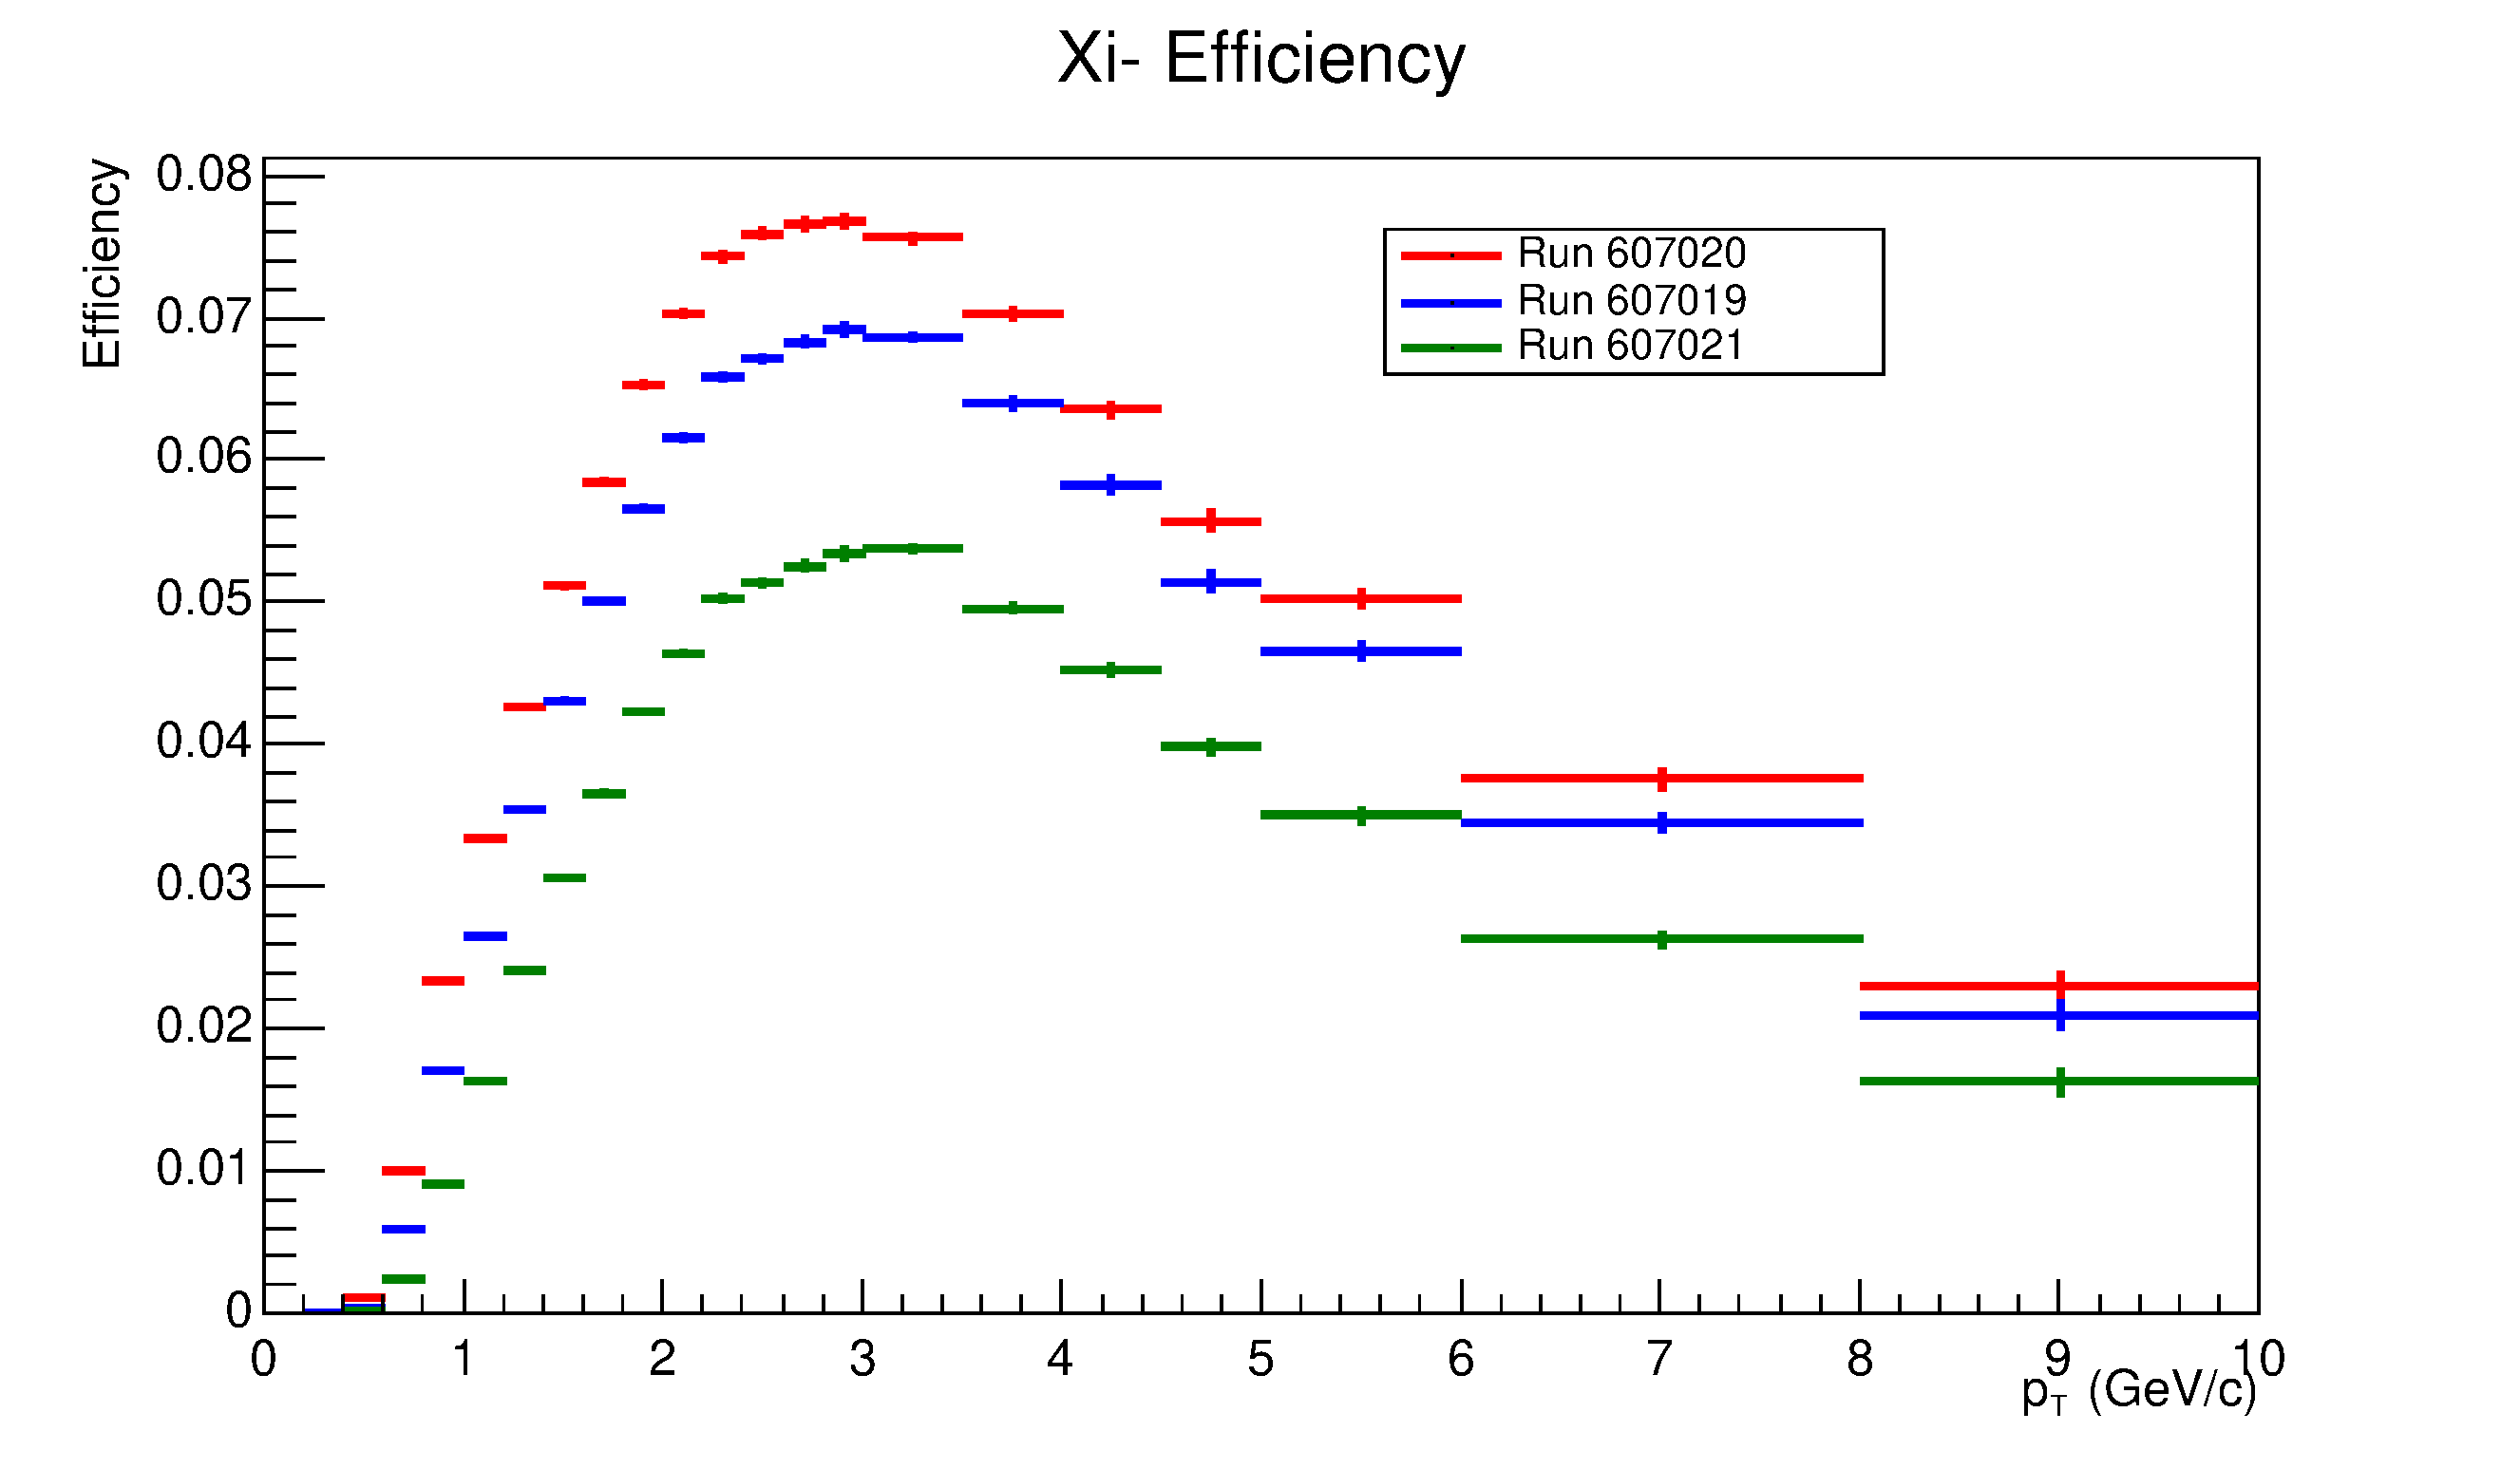
\includegraphics[width=.8\textwidth]{figures/Intermezzo/systematics/EffSpectraSys.pdf}
      \caption{Reconstruction efficiencies for the different systematic uncertainty variations.}
      \label{fig:EffSpectraSys}
    \end{figure}

    \begin{figure}[ht]
      \centering
      \includegraphics[width=.8\textwidth]{figures/Intermezzo/systematics/spectra_ratio_sysvars.pdf}
      \caption{Ratio of the \Xi\ \pt\ spectra for the different systematic uncertainty variations. The vertical bars represent the statistical uncertainties subtracted in quadrature, assuming they are fully correlated between the variations.}
      \label{fig:SpectraRatioSys}
    \end{figure}

    \rs{I'll make the plots nicer for the thesis}

  \subsection{Other sources of systematic uncertainties}
    \rs{to be expanded later}
    We take the material budget uncertainty from the previous analysis, see Figure \ref{fig:MaterialBudget}. 

    \begin{figure}
      \centering
      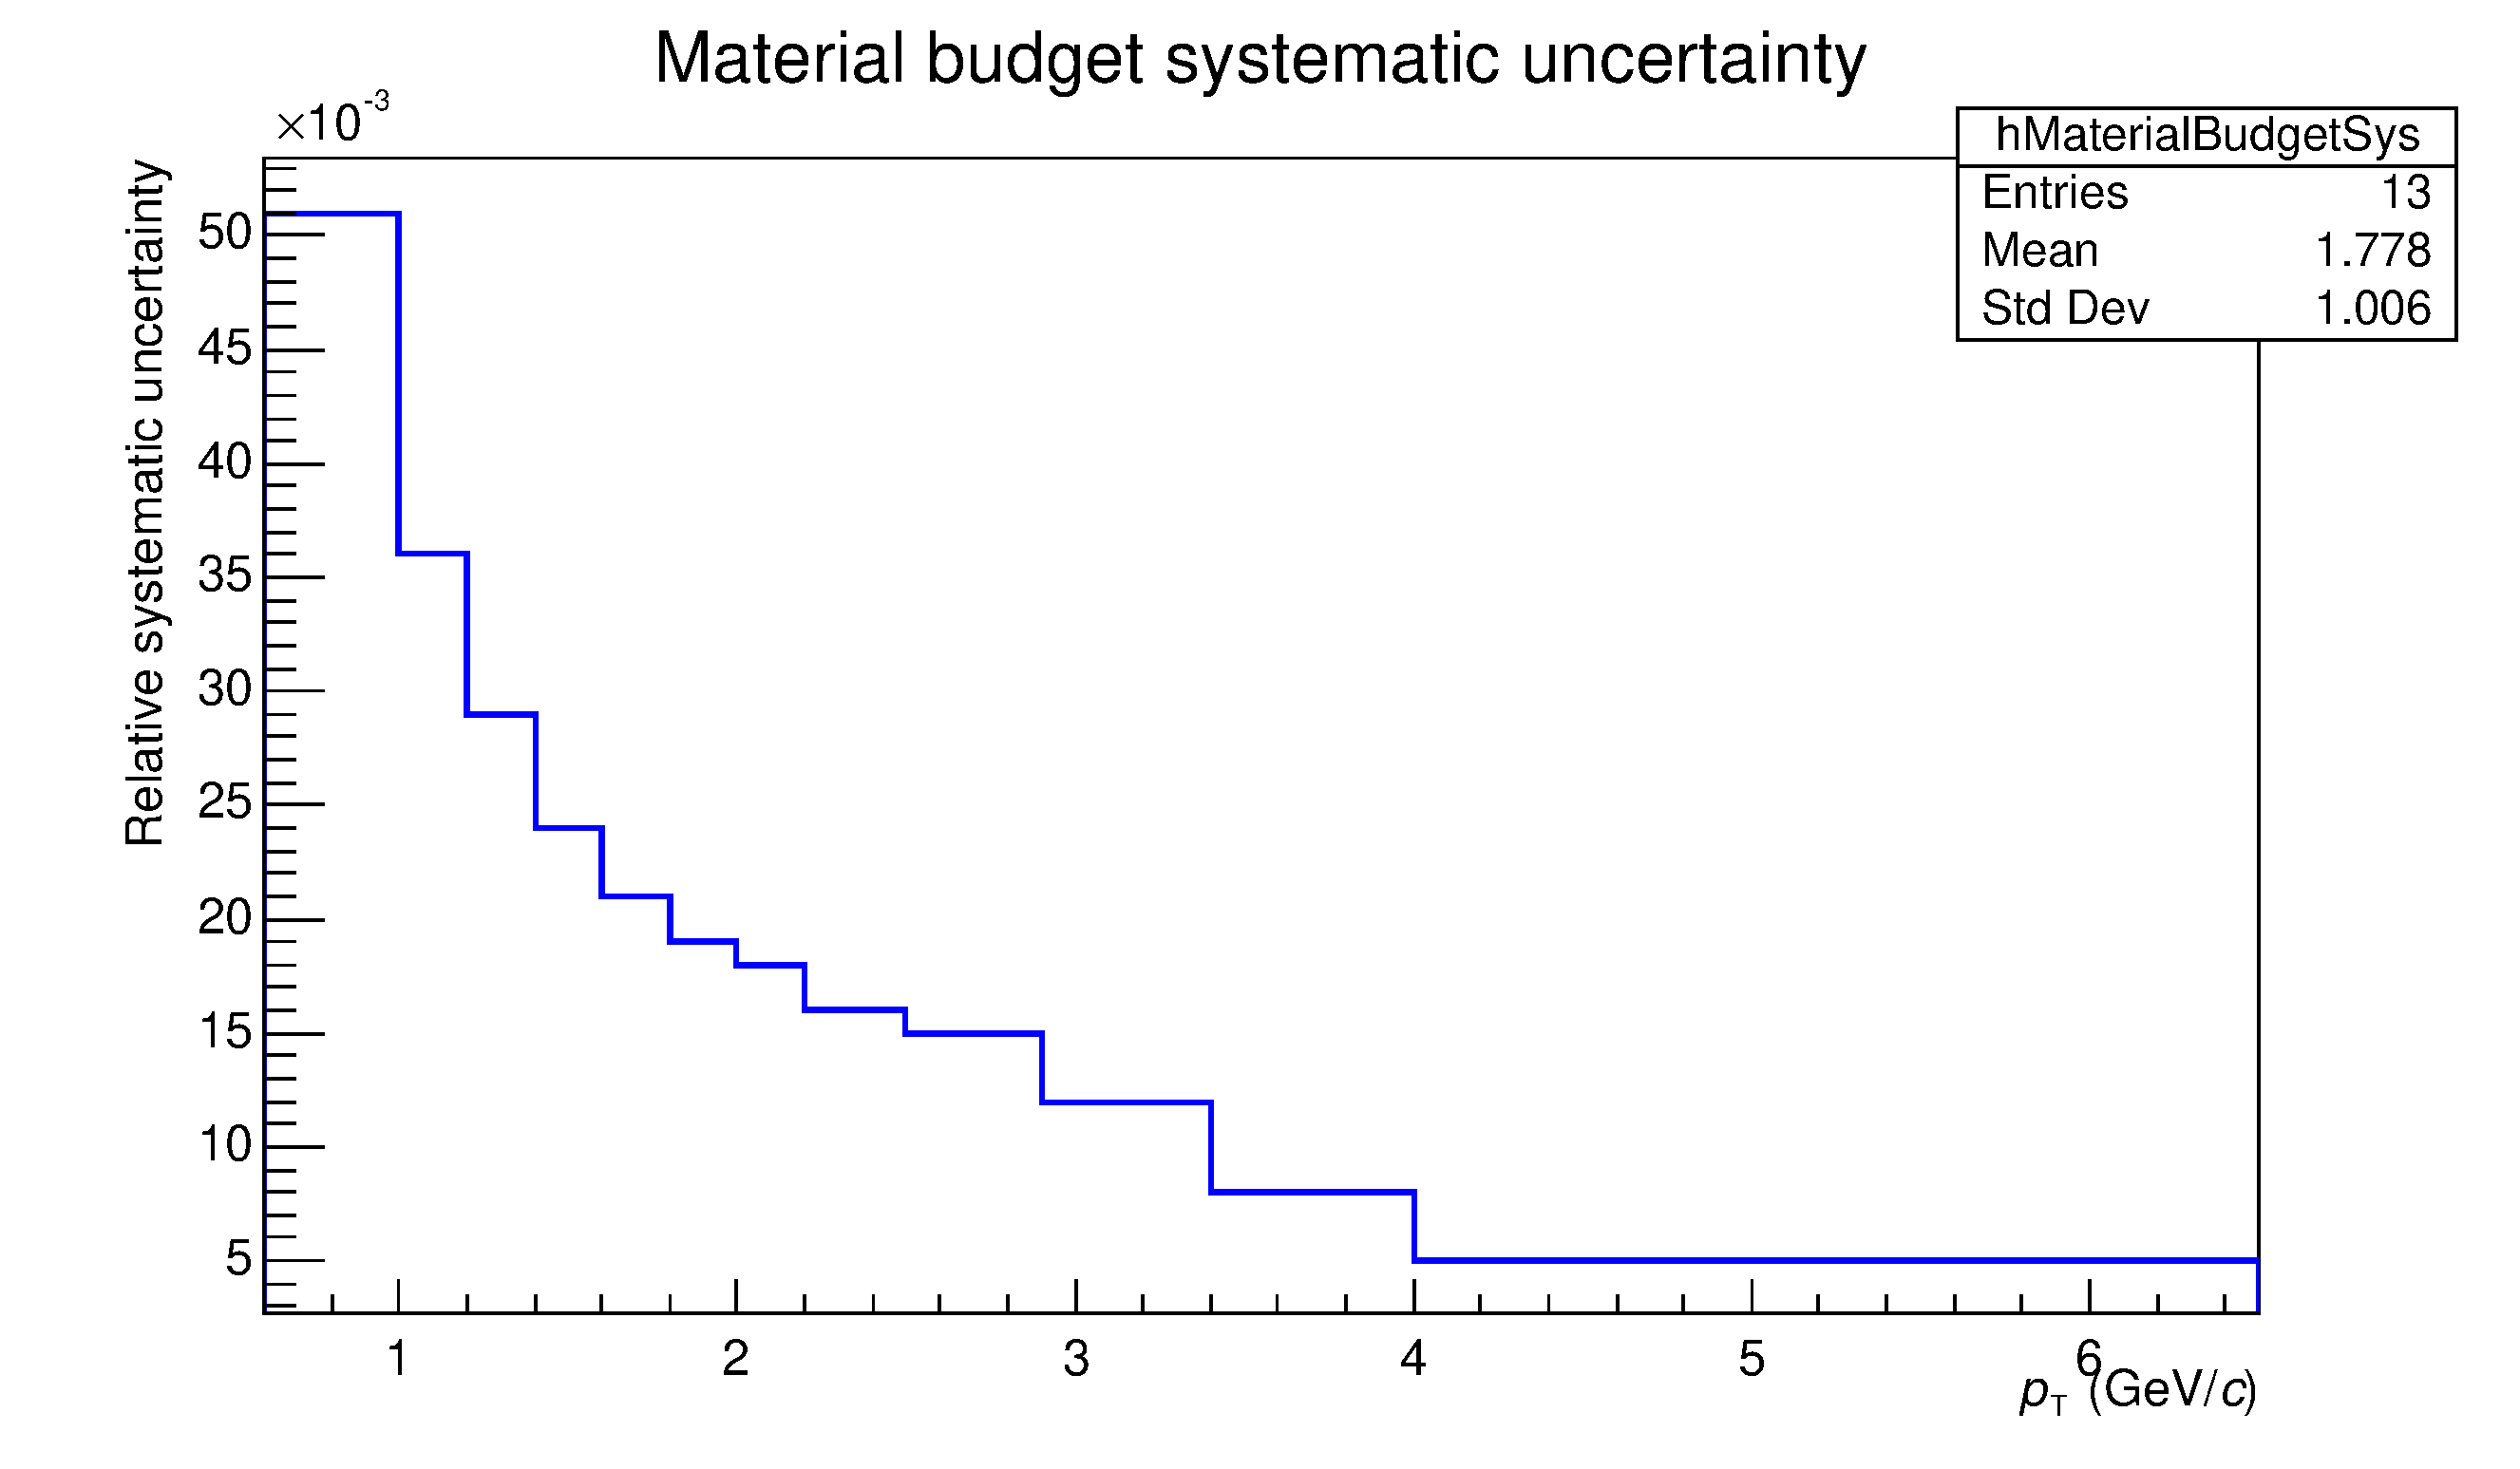
\includegraphics[width=.8\textwidth]{figures/Intermezzo/systematics/MaterialBudgetTemp.pdf}
      \caption{Material budget uncertainty as a function of \pt, taken from the previous analysis.}
      \label{fig:MaterialBudget}
    \end{figure}

    \rs{maybe mention background subtraction? varying bkg fit function or fit range. }

\section{Results for single \texorpdfstring{\Xi}{Xi} spectra}
  \label{sec:intermezzo:results}
  The \Xi\ baryon transverse momentum distributions calculated according to Equation \ref{eq:single_spectra} are shown in the top panel of Figure \ref{fig:SpectraRatio}, where they are compared to the results of the analysis performed on Run 2 data.\cite{Run2Spectra} The bottom panel of Figure \ref{fig:SpectraRatio} shows the ratio of the two spectra, where the vertical bars represent the statistical uncertainties added in quadrature. The results show a good agreement between the two analyses. It seems that we estimate the yield to be slightly lower than the previous analysis, but still well within the systematic uncertainties. 
  
  The only exception is the lowest \pt\ bin, which can be explained by considering the effect of a pseudorapidity window $|\eta| < 0.8$ in combination with a rapidity window $|y| < 0.5$. In order to compare with previous analyses, we apply this rapidity selection on top of the pseudorapidity selection that we use to be consistent with the correlation analysis. This leads to an incorrect efficiency correction in the range where $|\eta| > 0.8$ and $|y| < 0.5$, which for the \Xi\ baryon occurs at $\pt \approx 0.96$ GeV/$c$.\footnote{As $|\eta| = 0.8$ corresponds to the edge of our detector, we don't expect a large increase of yield beyond this range. However, in the efficiency correction we should not remove cascades that are generated within $|y| < 0.5$ but reconstructed with $|\eta| > 0.8$. Doing this leads to an overestimation of the efficiency, and therefor an underestimation of the yield, as can be seen in the lowest \pt\ bin.}

  \begin{figure}[ht]
    \centering
    \includegraphics[width=.8\textwidth]{figures/Intermezzo/spectra_ratio.pdf}
    \caption{\Xi\ baryon yields as a function of \pt. Results of this analysis are compared to the results of the analysis performed on Run 2 data.\cite{Run2Spectra} Systematic errors are displayed as shaded boxes, statistical errors as vertical bars. The ratio of the two spectra is shown in the bottom panel, here the vertical bars represent the statistical uncertainties added in quadrature.}
    \label{fig:SpectraRatio}
  \end{figure}
  \rs{this is a placeholder, I'll add the sys. uncertainties for this analysis after I run on the full dataset.}

\section{TEMP: 2 ways to determine the systematics for the correlation analysis}

  In any case I'll take 3\% as an estimate of the material budget uncertainty. 

  \subsection{Take the systematics from the spectra analysis}

    This comes down to a flat 1.5\% uncertainty from the topological selection criteria, and a 3\% uncertainty from the material budget, added in quadrature. We can even take the topological uncertainty to be lower than 1.5\% - as the material budget uncertainty is the dominant source of systematic uncertainty, the exact value of the topological selection criteria uncertainty doesn't have a large effect on the total systematic uncertainty.

    For the OS-SS we then compute it using the absolute values of the systematic uncertainties on the OS and SS respectively, assuming they are fully correlated. 

  \subsection{Take the systematics from the correlation analysis}

    

    